\section{Running Example}
\label{sec:example}
We present a running example of a simplified sensor system in a Pressurized Water Reactor (PWR). In a typical PWR, the core inside of the reactor vessel produces heat. Pressurized water in the primary coolant loop carries the heat to the steam generator. Within the steam generator, heat from the primary coolant loop vaporizes the water in a secondary loop, producing steam. The steamline directs the steam to the main turbine, causing it to turn the turbine generator, which produces electricity. There are a few important factors that must be considered during safety assessment and system design. An unsafe climb in temperature can cause high pressure and hence pipe rupture, and high levels of radiation could indicate a leak of primary coolant. 

\begin{figure*}[h!]
	%\vspace{-2em}
	\begin{center}
		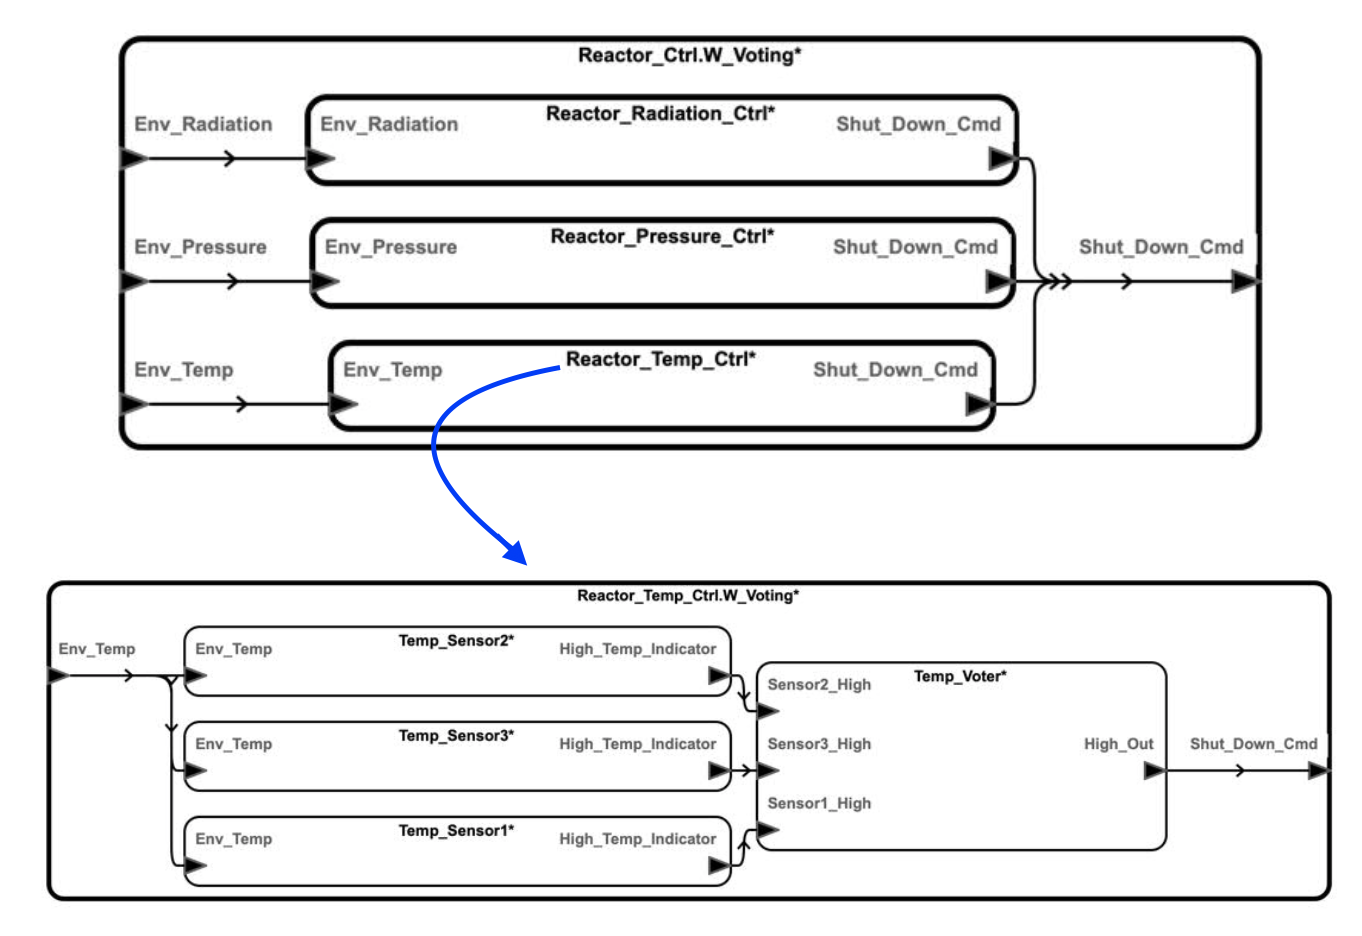
\includegraphics[width=0.8\textwidth]{images/sensorSysAADL.png}
	\end{center}
	\vspace{-2em}
	\caption{PWR Sensor System}
	\label{fig:sensorSys}
	%\vspace{-2em}
\end{figure*}

The following sensor system can be thought of as a subsystem within a PWR that monitors these factors. A diagram of the model is shown in Figure~\ref{fig:sensorSys} and represents a simplified version of a safety critical system. The temperature subsystem details are shown at the bottom of Figure~\ref{fig:sensorSys}; each of the subsystems have a similar architecture.

The subsystems each contain three sensors that monitor pressure, temperature, and radiation. Environmental inputs are fed into each sensor in the model and the redundant sensors monitor temperature, pressure, or radiation respectively. If temperature, pressure, or radiation is too high, a shut down command is sent from the sensors to the parent components. 

The temperature, pressure, and radiation sensor subsystems each contan three associated sensors for redundancy. Each sensor reports the associated environmental condition to a majority voter component. If the majority of the sensors reports high, a shut down command is sent to the subsystem. If any subsystem reports a shut down command, the top level system will shut down. Pressure, radiation, and temperature all have associated thresholds for high values which we refer to as $T_p$, $T_r$, and $T_t$ respectively. The safety property $P$ of interest in this system is: \emph{shut down when we should} and is reflected by the shut down command at the top level ({\em Shut\_Down\_Cmd}):

\begin{equation*}
\begin{split}
Shut\_Down\_Cmd &=  Env\_Temp > THRESHOLD\\
  & \lor  Env\_Pressure > THRESHOLD\\
  & \lor Env\_Radiation > THRESHOLD
\end{split}
\end{equation*}

For reference throughout this paper, we provide Figure~\ref{fig:sensorSysContracts} which shows the guarantees and faults of interest for this running example. 

\begin{figure*}[h!]
	%\vspace{-2em}
	\begin{center}
		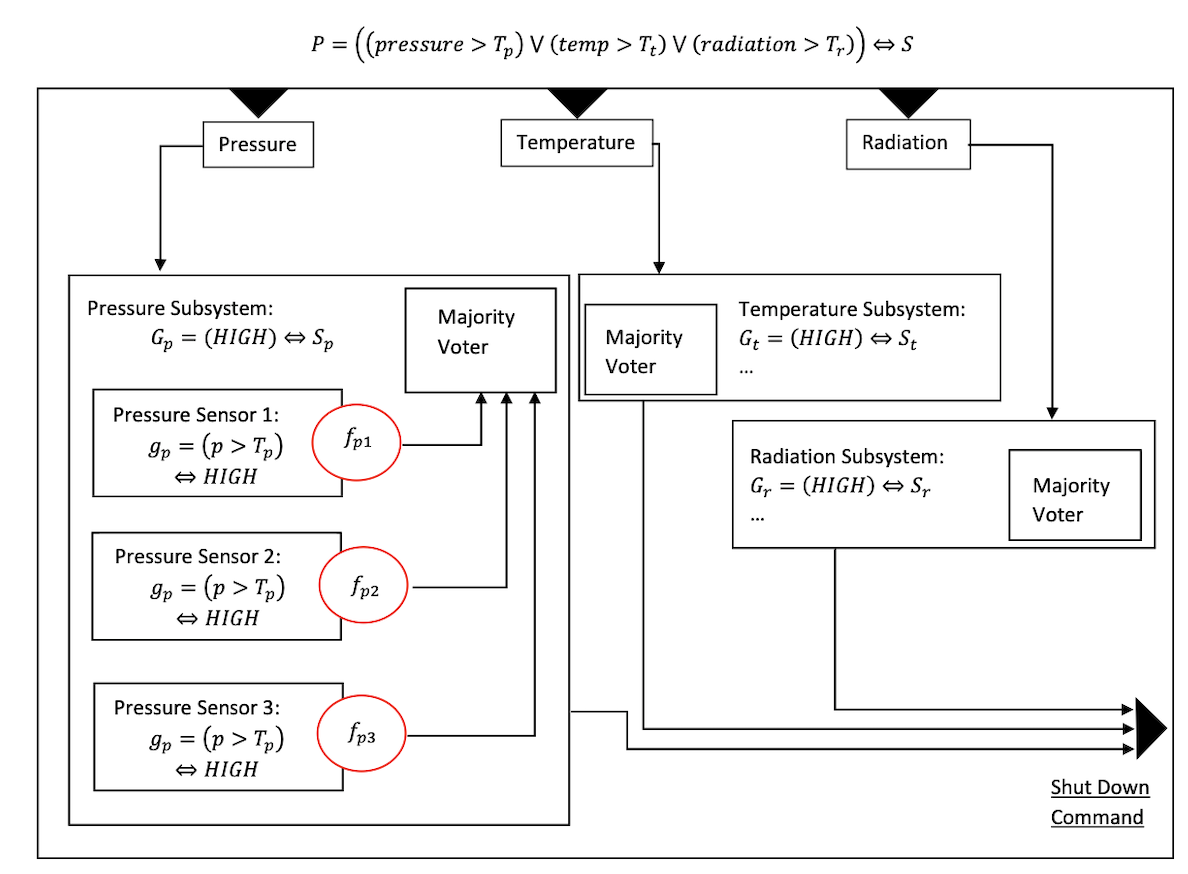
\includegraphics[width=1.0\textwidth, trim={0 7.5cm 0 0},clip]{images/PWRFigureContracts.png}
	\end{center}
	\vspace{-6em}
	\caption{Sensor System Nominal and Fault Model Details}
	\label{fig:sensorSysContracts}
	%\vspace{-2em}
\end{figure*}

Note: the thresholds vary for pressure, temperature, and radiation. These are given as constants $T_p$, $T_t$, and $T_r$ respectively. The top level shut down command is given as $S$ and each sensor subsystem provides their own shutdown command, $S_p$ for example.  The faults are shown as ``fail low" which correspond to the environmental condition being high, but the sensor reports safe ranges. We do not show all guarantees and assumptions that are in the model, but only the ones of interest for the illustration. 

Initially, the faults that are of interest in this system are unconstrained guarantees. When a guarantee becomes unconstrained, the output over which it is defined may be faulty. For our purposes in the next section, this situation is what we want to explore. 

\begin{comment}
\subsection{PWR Fault Model}
The faults that are of interest in this example system are any one of the sensors failing high or low. If sensors report high and a shut down command is sent, we shut down when we should not. On the other hand, if sensors report low when it should be high, a shut down command is not sent and we do not shut down when we should. From the perspective of safety, a false report of low temperature is the main concern. For simplification in this paper, we focus on the failures when sensors report low when they should not.

A fault is defined for each sensor in the system using the safety annex. An example of a temperature sensor fault stuck at high is shown in Figure~\ref{fig:tempSensorFault}.

\begin{figure*}[h!]
	%\vspace{-2em}
	\begin{center}
		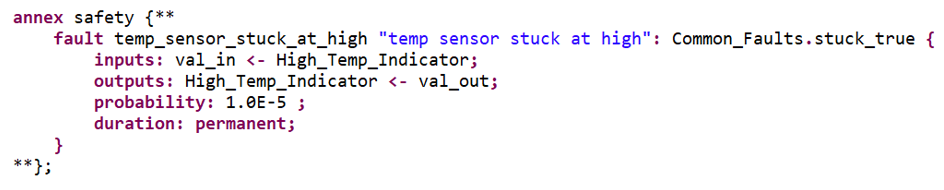
\includegraphics[width=0.9\textwidth]{images/tempSensorFault.PNG}
	\end{center}
	\vspace{-2em}
	\caption{Fault on Temperature Sensor Defined in the Safety Annex for AADL}
	\label{fig:tempSensorFault}
	\vspace{-2em}
\end{figure*}

The Safety Annex provides a way to weave the faults into the nominal model by use of the \emph{inputs} and \emph{outputs} keywords. This allows users to define a fault and attach it to the output of a component. The fault shown in Figure~\ref{fig:tempSensorFault} is defined to be a {\em permanent} fault and has probability of occurrence set at $1.0 \times 10^{-5}$. If the fault is active, the error can possibly violate the guarantees of this component or the assumptions of downstream components~\cite{stewart2020safety}. The activation of a fault is not up to the user, but instead left up to the model checker, JKind, to determine if the activation of this fault will contribute to a violation of higher level guarantees. If so, it can be activated during the analysis.





\begin{center}
\resizebox{0.5\textwidth}{!}{%
    \begin{tabular}{ | c | c | c |}
      \hline
      \thead{Component} & \thead{Layer of Analysis} & \thead{Guarantee}\\
      \hline
      ReactorSys & Top &  \makecell{Safety Property $P$: \\ $((temp$ $>$ $T_t)$ $\lor$ $ (pressure$ $>$ $ T_p)$  $\lor$ $ (radiation$ $>$ $ T_r))$ \\ $\iff SHUTDOWN$}    \\
      \hline
      TempSys & Leaf  &  \makecell{Guarantee $G_t$: \\  $temp$ $>$ $ T_t \iff SHUTDOWN$}   \\
      \hline
      PressureSys & Leaf  &  \makecell{Guarantee $G_p$: \\ $pressure$ $>$ $ T_p \iff SHUTDOWN$}    \\
	\hline
      RadiationSys & Leaf  &  \makecell{Guarantee $G_r$: \\ $radiation$ $>$ $ T_r \iff SHUTDOWN$}   \\
      \hline
    \end{tabular}}
  \end{center}

\begin{center}
\resizebox{0.5\textwidth}{!}{%
    \begin{tabular}{ | c | c | c |}
      \hline
      \thead{Component} & \thead{Layer of Architecture} & \thead{Faults}\\
      \hline
      Temp Sensors (3) & \makecell{Leaf \\ Components} & \makecell{$f_{t}$: fail low}  \\
      \hline
	Pressure Sensors (3) & \makecell{Leaf \\ Components} & \makecell{$f_{p}$: fail low}  \\
      \hline
	Radiation Sensors (3) & \makecell{Leaf \\ Components} & \makecell{$f_{r}$: fail low}  \\
      \hline
    \end{tabular}}
  \end{center}



\subsection{Using this Example in the Generation of Minimal Cut Sets}
Step by step, we outline how minimal cut sets are generated through the \aivcalg algorithm using the sensor system as an example. For ease of reference, a table is provided giving model elements of interest in the sensor example. We refer to these throughout this section. Note: the thresholds vary for pressure, temperature, and radiation. These are given as constants $T_p$, $T_t$, and $T_r$ respectively. We also do not list all guarantees and assumptions that are in the model, but only the ones of interest for this analysis.

\begin{center}
\resizebox{\textwidth}{!}{%
    \begin{tabular}{ | c | c | c |}
      \hline
      \thead{Component} & \thead{Layer of Analysis} & \thead{Guarantee}\\
      \hline
      ReactorSys & Top &  \makecell{Safety Property $P$: \\ $((temp$ $>$ $T_t)$ $\lor$ $ (pressure$ $>$ $ T_p)$  $\lor$ $ (radiation$ $>$ $ T_r))$ \\ $\iff SHUTDOWN$}    \\
      \hline
      TempSys & Leaf  &  \makecell{Guarantee $g_t$: \\  $temp$ $>$ $ T_t \iff SHUTDOWN$}   \\
      \hline
      PressureSys & Leaf  &  \makecell{Guarantee $g_p$: \\ $pressure$ $>$ $ T_p \iff SHUTDOWN$}    \\
	\hline
      RadiationSys & Leaf  &  \makecell{Guarantee $g_r$: \\ $radiation$ $>$ $ T_r \iff SHUTDOWN$}   \\
      \hline
    \end{tabular}}
  \end{center}

\begin{center}
%\resizebox{\textwidth}{!}{%
    \begin{tabular}{ | c | c | c |}
      \hline
      \thead{Component} & \thead{Layer of Architecture} & \thead{Faults}\\
      \hline
      Temp Sensors (3) & \makecell{Leaf \\ Components} & \makecell{$f_{t}$: fail low}  \\
      \hline
	Pressure Sensors (3) & \makecell{Leaf \\ Components} & \makecell{$f_{p}$: fail low}  \\
      \hline
	Radiation Sensors (3) & \makecell{Leaf \\ Components} & \makecell{$f_{r}$: fail low}  \\
      \hline
    \end{tabular}
  \end{center}

The first two steps of this process are performed top down in conjunction with JKind analysis over a program. Thus, the top layer is analyzed first, then the next and so on. Steps 3 and 4 proceed after all MIVCs for each layer have been generated. We walk through this sensor system example in this fashion. 

\textbf{Step 1a: Preprocessing top layer.} The preprocessing step inserts specific MIVC elements into the Lustre program. The MIVC elements are the model elements considered in the constraint system for a given property. The Safety Annex provides the means to define a fault over the output of a component. This fault is given an unassigned \emph{trigger} Boolean literal in Lustre. If the trigger literal is true, the output of the component is changed. If not, the output remains equivalent to the nominal output of this component~\cite{stewart2020safety, Stewart17:IMBSA}. This trigger in Lustre is called a \emph{fault activation literal}. The IVC elements required in order to perform this transformation are these fault activation literals as well as guarantees. The basic rules used to insert these additional literals into Lustre depend on the analysis layer of that is being formed in Lustre and are as follows. 
\begin{itemize}
\item Leaf layer of analysis: only fault activation literals are added.
\item Middle or top layers: guarantees are added and if a direct subcomponent is a leaf component of the architecture and faults are defined on its outputs, then these faults are also added.
\end{itemize}

At the top level, guarantees of the sensor subsystems are the IVC elements.
$$\boxed{g_t, g_p, g_r}$$

There are distinct constraint systems, one for each property being proved. In this system at the top layer, there is a single property $P$; this results in the following constraint system. 
$$\boxed{C = \{g_t, g_p, g_r, \neg P\}}$$

\textbf{Step 2a: Generate all MIVCs for the constraint system at the top layer.} In order to prove $P$, all three guarantees from the sensor subsystem level are required. 
$$\boxed{MIVC(P) = \{g_t, g_p, g_r\}}$$. 

\textbf{Step 1b: Preprocessing leaf layer.} Model elements for the IVC algorithm consideration are the faults for each sensor, for instance temperature sensors:
$$\boxed{f_{t1}, f_{t2}, f_{t3}}$$ 

The resulting constraint system for the temperature sensor subsystem layer is:
$$\boxed{C = \{\neg f_{t1}, \neg f_{t2}, \neg f_{t3}, \neg g_t\}}$$

\textbf{Step 2b: Generate all MIVCs for the constraint system at the leaf layer.} Due to the majority voting mechanism, the MIVCs show all possible pairs of faults restricted to \emph{false}. This means, if any combination of two faults do not occur, then the guarantees at the temperature sensor subsystem level are satisfied. 
$$\boxed{
	\begin{aligned}
		MIVC_1(g_t) = \{\neg f_{t1}, \neg f_{t2}\} \\
		MIVC_2(g_t) = \{\neg f_{t1}, \neg f_{t3}\} \\
		MIVC_3(g_t) = \{\neg f_{t2}, \neg f_{t3}\}
	\end{aligned}
}$$

At this point, all MIVCs have been successfully generated (which is a requirement of the following algorithms) and we can move on to the generation of minimal cut sets. 

\textbf{Step 3a: Generate MCSs using a hitting set algorithm at the top layer.} Our single MIVC in this case will reveal three associated MCSs. (Notice: $MCS_1 \cap MIVC(P) \neq \emptyset$, and same for $MCS_2$ and $MCS_3$, thus these are hitting sets.)
 $$\boxed{
	\begin{aligned}
		MCS_1(top) = \{g_t\} \\
		MCS_2(top) = \{g_p\} \\
		MCS_3(top) = \{g_r\}
	\end{aligned}
}$$

\textbf{Step 4a: Transform MCSs into MinCutSets at the top layer.} Given that only guarantees are found in the MCSs at this layer, recursion is used to find the faults that cause violation of these guarantees. Using this recursion on $MCS_1$, we show the process further. 

\textbf{Step 3b: Generate MCSs using a hitting set algorithm at the leaf layer.} In step 2b, we found all MIVCs for the contract $g_t$ and send these to the hitting set algorithm. The resulting MCSs are: 
 $$\boxed{
	\begin{aligned}
		MCS_1(leaf) = \{\neg f_{t1}, \neg f_{t2}\} \\
		MCS_2(leaf) = \{\neg f_{t1}, \neg f_{t3}\} \\
		MCS_3(leaf) = \{\neg f_{t2}, \neg f_{t3}\}
	\end{aligned}
}$$

Only constrained faults are found in these MCSs, so we simply remove those constraints and have found the MinCutSets for the contracts $g_t$. These are returned and replace this contract in the top layer $MCS_1(top)$. Here is the end result for $MCS_1(top)$; this can be understood as three of the total minimal cut sets for $P$. 

\begin{equation*}
MCS_1(top) \rightarrow \left\{ \,
\begin{IEEEeqnarraybox}[][c]{l?s}
\IEEEstrut
MinCutSet_1(P) = \{f_{t1}, f_{t2}\}, \\
MinCutSet_2(P) = \{f_{t1},  f_{t3}\}, \\
MinCutSet_3(P) = \{f_{t2}, f_{t3}\}
\IEEEstrut
\end{IEEEeqnarraybox}
\right.
\end{equation*}

After all replacements have been made, we are left with all minimal cut sets for the property of interest ($P$ in this example). 

\end{comment}









